\section{Results}\label{sec:results}

This section provides the results of the CPU vs. GPU comparison, as well as the performance of the Transformer model on the translation task.

\subsection{GPU versus CPU Training}

\cref{tab:comparison} illustrates the results of the performance comparison between CPU and GPU training.
The GPU significantly accelerates the overall training process by a factor of 8.07.
Accordingly, the GPU processes a single epoch, as well as a forward pass, faster by approximately the same margin.
The GPU achieves the most significant speed-up (20x) during the backward pass.
This highlights the GPU's superior efficiency in handling computationally expensive tasks, such as gradient computation, which heavily rely on parallelized matrix calculations.
Surprisingly, the GPU uses 38 times less memory per epoch compared to the CPU, which can mainly be attributed to the small batch size of 32 for both setups.\\
Due to approaching deadlines and long queues on the high performance cluster (HPC), I postpone further optimizations of the GPU codebase.
For instance, offloading BLEU score calculations to the CPU, combined with mixed-precision training and other optimizations, can approximately halve overall training time--a speedup that has been observed in practical 11.\\
\begin{table}[ht]
    \centering
    \begin{tabular}{lccc}
        \toprule
        \textbf{Metric} & \textbf{CPU} & \textbf{GPU} & \textbf{CPU to GPU Ratio} \\
        \midrule
        Training time (hours)       & 3.0017 & 0.3717 & 8.07 \\
        Avg. Epoch times (seconds)       & 2161.24 & 267.63 & 8.07 \\
        Avg. Forward pass times (seconds)& 0.0770 & 0.0088 & 8.75 \\
        Avg. Backward pass time (seconds)& 0.2020 & 0.0101 & 20 \\
        Avg. Single step time (seconds)  & 0.2790 & 0.0189 & 14.76  \\
        Allocated memory per epoch (MB)       & 32998.0  & 865.91 & 38.1 \\
        \bottomrule
    \end{tabular}
    \caption{Performance comparison of CPU vs. GPU}
    \label{tab:comparison}
\end{table}
While the performance benefits speak for themselves, GPU training entails some disadvantages.
Working on the HPC, I experienced long queues before the jobs could start, as well as complexity in setting up the code and accompanying libraries to run on the GPU nodes.
This results in longer feedback cycles because each attempt requires submitting a new job and waiting.
If errors occur, they only got discovered after the job queue processed the experiment, further extending debugging time.
Additionally, estimating the memory resources for optimizing throughput was time-consuming and often required trial and error, especially without easy access to a GPU for testing.

\clearpage
\subsection{Machine Translation}
\cref{fig:bleu} shows that on the WMT German-to-English translation task, the Transformer model reaches a BLEU score of around 0.34 with a length ratio of 0.99 on the validation set, which implies solid, coherent translations.
Training took approximately 11.5 hours.


\begin{figure}[ht]
    \begin{center}
        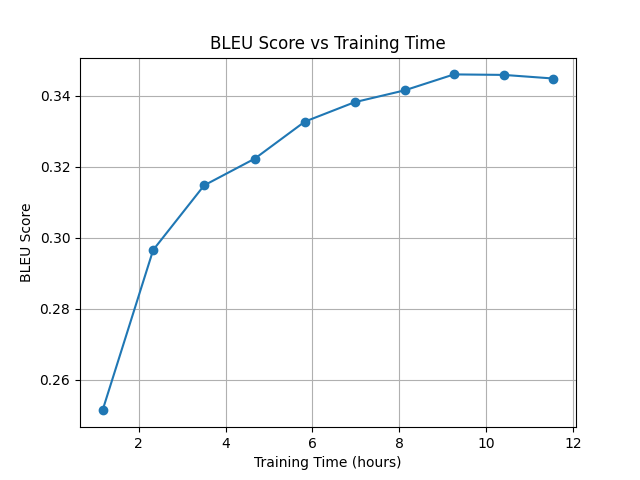
\includegraphics[width=\textwidth]{figures/bleu_score_val_20250129_142747.png}
    \end{center}
    \caption{The BLEU score is calculated on the validation set after each epoch. It approaches a value of around 0.34.}
    \label{fig:bleu}
\end{figure}
Word count: 2282
